% !TEX TS-program = knitr
\documentclass[handout]{beamer}\usepackage{graphicx, color}
%% maxwidth is the original width if it is less than linewidth
%% otherwise use linewidth (to make sure the graphics do not exceed the margin)
\makeatletter
\def\maxwidth{ %
  \ifdim\Gin@nat@width>\linewidth
    \linewidth
  \else
    \Gin@nat@width
  \fi
}
\makeatother

\IfFileExists{upquote.sty}{\usepackage{upquote}}{}
\definecolor{fgcolor}{rgb}{0.2, 0.2, 0.2}
\newcommand{\hlnumber}[1]{\textcolor[rgb]{0,0,0}{#1}}%
\newcommand{\hlfunctioncall}[1]{\textcolor[rgb]{0.501960784313725,0,0.329411764705882}{\textbf{#1}}}%
\newcommand{\hlstring}[1]{\textcolor[rgb]{0.6,0.6,1}{#1}}%
\newcommand{\hlkeyword}[1]{\textcolor[rgb]{0,0,0}{\textbf{#1}}}%
\newcommand{\hlargument}[1]{\textcolor[rgb]{0.690196078431373,0.250980392156863,0.0196078431372549}{#1}}%
\newcommand{\hlcomment}[1]{\textcolor[rgb]{0.180392156862745,0.6,0.341176470588235}{#1}}%
\newcommand{\hlroxygencomment}[1]{\textcolor[rgb]{0.43921568627451,0.47843137254902,0.701960784313725}{#1}}%
\newcommand{\hlformalargs}[1]{\textcolor[rgb]{0.690196078431373,0.250980392156863,0.0196078431372549}{#1}}%
\newcommand{\hleqformalargs}[1]{\textcolor[rgb]{0.690196078431373,0.250980392156863,0.0196078431372549}{#1}}%
\newcommand{\hlassignement}[1]{\textcolor[rgb]{0,0,0}{\textbf{#1}}}%
\newcommand{\hlpackage}[1]{\textcolor[rgb]{0.588235294117647,0.709803921568627,0.145098039215686}{#1}}%
\newcommand{\hlslot}[1]{\textit{#1}}%
\newcommand{\hlsymbol}[1]{\textcolor[rgb]{0,0,0}{#1}}%
\newcommand{\hlprompt}[1]{\textcolor[rgb]{0.2,0.2,0.2}{#1}}%

\usepackage{framed}
\makeatletter
\newenvironment{kframe}{%
 \def\at@end@of@kframe{}%
 \ifinner\ifhmode%
  \def\at@end@of@kframe{\end{minipage}}%
  \begin{minipage}{\columnwidth}%
 \fi\fi%
 \def\FrameCommand##1{\hskip\@totalleftmargin \hskip-\fboxsep
 \colorbox{shadecolor}{##1}\hskip-\fboxsep
     % There is no \\@totalrightmargin, so:
     \hskip-\linewidth \hskip-\@totalleftmargin \hskip\columnwidth}%
 \MakeFramed {\advance\hsize-\width
   \@totalleftmargin\z@ \linewidth\hsize
   \@setminipage}}%
 {\par\unskip\endMakeFramed%
 \at@end@of@kframe}
\makeatother

\definecolor{shadecolor}{rgb}{.97, .97, .97}
\definecolor{messagecolor}{rgb}{0, 0, 0}
\definecolor{warningcolor}{rgb}{1, 0, 1}
\definecolor{errorcolor}{rgb}{1, 0, 0}
\newenvironment{knitrout}{}{} % an empty environment to be redefined in TeX

\usepackage{alltt}
\newcommand{\answers}{1}

\setbeamercovered{dynamic}
\usetheme{Marburg}
\setbeamertemplate{navigation symbols}{} 
\setbeamertemplate{footline}
{
  \leavevmode%
  \hbox{%
  \begin{beamercolorbox}[wd=.333333\paperwidth,ht=2.25ex,dp=1ex,center]{author in head/foot}%
    \usebeamerfont{author in head/foot}\copyright $\ $ \insertshortauthor%~~\beamer@ifempty{\insertshortinstitute}{}{(\insertshortinstitute)}
  \end{beamercolorbox}%
  \begin{beamercolorbox}[wd=.333333\paperwidth,ht=2.25ex,dp=1ex,center]{title in head/foot}%
    \usebeamerfont{title in head/foot} \insertinstitute
  \end{beamercolorbox}%
  \begin{beamercolorbox}[wd=.333333\paperwidth,ht=2.25ex,dp=1ex,right]{date in head/foot}%
    \usebeamerfont{date in head/foot}\insertshortdate{}\hspace*{2em}
    \insertframenumber{} / \inserttotalframenumber\hspace*{2ex} 
  \end{beamercolorbox}}%
  \vskip0pt%
}{}

\usepackage{amsmath}
\usepackage{caption}
\usepackage{color}
\usepackage{enumerate}
\usepackage{listings}
\usepackage{hyperref}
\usepackage{mathrsfs}
\usepackage{natbib}
\usepackage{url}

\providecommand{\all}{\ \forall \ }
\providecommand{\bs}{\backslash}
\providecommand{\e}{\varepsilon}
\providecommand{\E}{\ \exists \ }
\providecommand{\lm}[2]{\lim_{#1 \rightarrow #2}}
\providecommand{\m}[1]{\mathbb{#1}}
\providecommand{\nv}{{}^{-1}}
\providecommand{\ov}[1]{\overline{#1}}
\providecommand{\p}{\newpage}
\providecommand{\q}{$\quad$ \newline}
\providecommand{\rt}{\rightarrow}
\providecommand{\Rt}{\Rightarrow}
\providecommand{\vc}[1]{\boldsymbol{#1}}
\providecommand{\wh}[1]{\widehat{#1}}

\hypersetup{colorlinks,linkcolor=,urlcolor=blue}
\numberwithin{equation}{section}

\definecolor{dkgreen}{rgb}{0,0.6,0}
\definecolor{gray}{rgb}{0.5,0.5,0.5}
\definecolor{mauve}{rgb}{0.58,0,0.82}

\lstset{ 
  language=C,                % the language of the code
  basicstyle= \footnotesize,           % the size of the fonts that are used for the code
  numberstyle= \tiny \color{white},  % the style that is used for the line-numbers
  stepnumber=2,                   % the step between two line-numbers. 
  numbersep=5pt,                  % how far the line-numbers are from the code
  backgroundcolor=\color{white},      % choose the background color. You must add \usepackage{color}
  showspaces=false,               % show spaces adding particular underscores
  showstringspaces=false,         % underline spaces within strings
  showtabs=false,                 % show tabs within strings adding particular underscores
  frame=lrb,                   % adds a frame around the code
  rulecolor=\color{black},        % if not set, the frame-color may be changed on line-breaks within not-black text 
  tabsize=2,                      % sets default tabsize to 2 spaces
  captionpos=t,                   % sets the caption-position 
  breaklines=true,                % sets automatic line breaking
  breakatwhitespace=false,        % sets if automatic breaks should only happen at whitespace
  %title=\lstname,                   % show the filename of files included with \lstinputlisting;
  keywordstyle=\color{blue},          % keyword style
  commentstyle=\color{gray},       % comment style
  stringstyle=\color{dkgreen},         % string literal style
  escapeinside={\%*}{*)},            % if you want to add LaTeX within your code
  morekeywords={*, ...},               % if you want to add more keywords to the set
  xleftmargin=0.053in, % left horizontal offset of caption box
  xrightmargin=-.03in % right horizontal offset of caption box
}

%\DeclareCaptionFont{white}{\color{white}}
%\DeclareCaptionFormat{listing}{\parbox{\textwidth}{\colorbox{gray}{\parbox{\textwidth}{#1#2#3}}\vskip-0.05in}}
%\captionsetup[lstlisting]{format = listing, labelfont = white, textfont = white}
%For caption-free listings, comment out the 3 lines above and uncomment the 2 lines below.
 \captionsetup{labelformat = empty, labelsep = none}
 \lstset{frame = single}





\title{Continuous Random Variables (Ch. 5.2)}
\author{Will Landau}
\date{Feb 21, 2013}
\institute{Iowa State University}

\begin{document}

\begin{frame}
\titlepage
 \end{frame}
 
 \AtBeginSection[]
{
   \begin{frame}
       \frametitle{Outline}
       \tableofcontents[currentsection]
   \end{frame}
}

\section{Introduction to Continuous Random Variables}

\begin{frame}
\frametitle{Continuous random variables}
\begin{itemize}
\pause \item Two types of random variables:
\begin{itemize}
\pause \item {\bf Discrete random variable}: one that can only take on a set of isolated points ($X$, $N$, and $S$).
\pause \item {\bf Continuous random variable}: one that can fall in an interval of real numbers ($T$ and $Z$). 
\end{itemize}
\pause \item Examples of continuous random variables:
\begin{itemize}
\pause \item $Z = $ the amount of torque required to loosen the next bolt (\emph{not} rounded).
\pause \item $T = $ the time you'll have to wait for the next bus home.
\pause \item $C = $ outdoor temperature at 3:17 PM tomorrow.
\pause \item $L =$ length of the next manufactured part.
\end{itemize}
\end{itemize}
\end{frame}



\begin{frame}
\frametitle{Continuous random variables}

\begin{itemize}
\pause \item $V$: \% yield of the next run of a chemical process.
\pause \item $Y$: \% yield of a \emph{better} process.
\pause \item How do we mathematically distinguish between $V$ and $Y$, given:
\begin{itemize}
\pause \item Each has the same range: $0\% \le V, Y \le 100\%$
\pause \item There are uncountably many possible values in this range.
\end{itemize} 
\pause \item We want to show that $Y$ tends to take on higher \% yield values than $V$.
\end{itemize}
\end{frame}

\begin{frame}
\frametitle{$V$ and $Y$ have \emph{continuous} probability distributions}

\begin{knitrout}
\definecolor{shadecolor}{rgb}{0.969, 0.969, 0.969}\color{fgcolor}
\includegraphics[width=\maxwidth]{figure/unnamed-chunk-2} 

\end{knitrout}

\begin{itemize}
\pause \item The heights of these curves are not themselves probabilities.
\pause \item However, the the curves tell us that process $Y$ will yield more product per run on average than process $X$.
\end{itemize}
\end{frame}

\begin{frame}
\frametitle{A generic probability density function (pdf)}
\setkeys{Gin}{width=1\textwidth} 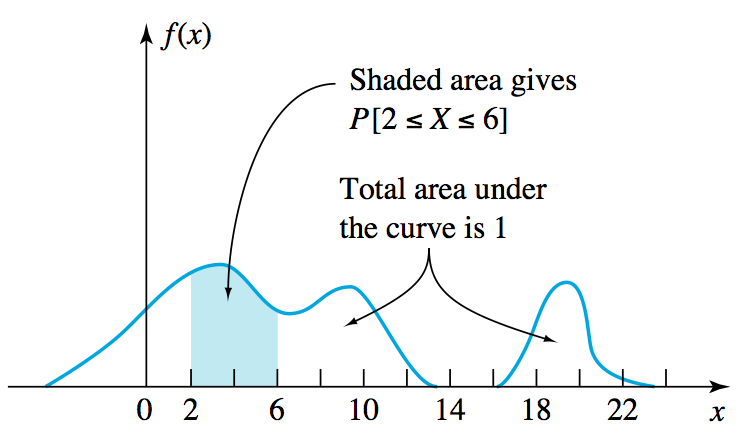
\includegraphics{../../fig/genpdf.png}

\end{frame}


\section{Probability Density Functions}

\begin{frame}
\frametitle{Definition: probability density function (pdf)}
\begin{itemize}
\pause \item A {\bf probability density function (pdf)} of a continuous random variable $X$ is a function $f(x)$ with:
\begin{align*}
&\uncover<3->{f(x)   \ge 0 \text{ for all }x.} \\
&\uncover<4->{\int_{- \infty}^\infty f(x) dx = 1} \\
&\uncover<5->{P(a \le X \le b) = \int_a^b f(x) dx, \ a \le b}
\end{align*}
\uncover<6->{ \item The pdf is the continuous analogue of a discrete random variable's probability mass function.}
\end{itemize}
\end{frame}


%\begin{frame}
%\frametitle{Example: measuring gravity}
%\begin{center}
%\setkeys{Gin}{width=.6\textwidth} 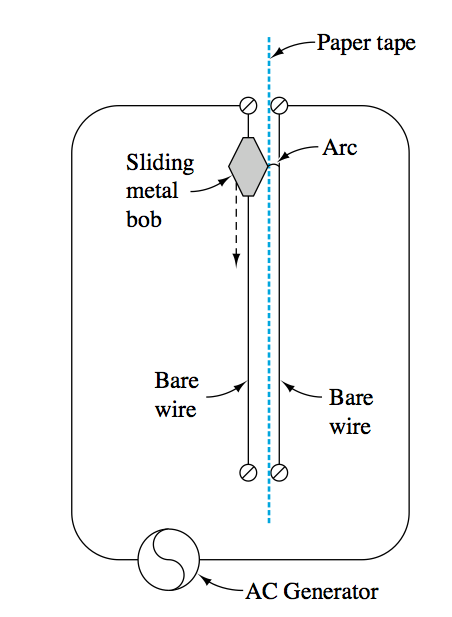
\includegraphics{../../fig/gravityschem.png}
%\end{center}
%\end{frame}

%\begin{frame}
%\frametitle{Example: measuring gravity}
%\begin{itemize}
%\item As the bob drops,  an electric arc shoots from the bob to the opposite wire every $60 \nv$ s, marking a burnt spot on the paper in between. 
%\item The displacement between the very top and the position of the bob at time $t$ is assumed to be:
%\begin{align*}
%d = \frac{1}{2} g t^2
%\end{align*}
%\item Let $Y$ be the elapsed time (in seconds) from the bob release until the first arc.
%\begin{itemize}
%\item The bob is released by hand, asynchronously with the 
%\end{itemize}
%\end{itemize}
%\end{frame}

\begin{frame}
\frametitle{Example} \small
\begin{itemize}
\pause \item Let $Y$ be the time delay (s) between a 60 Hz AC circuit and the movement of a motor on a different circuit.
\pause \item Say $Y$ has a density of the form:
\begin{align*}
\uncover<4->{f(y) = \begin{cases}
c & 0 < y < \frac{1}{60}\\
0 & \text{otherwise}
\end{cases}}
\end{align*}
\uncover<5->{we say that $Y$ has a Uniform(0, 1/60) distribution.}
\uncover<6->{\item $f(y)$ must integrate to 1:}
\begin{align*}
\uncover<7->{1 = \int_{- \infty}^\infty f(y) dy}  \uncover<8->{= \int_{- \infty}^0 0 dy  + \int_0^{1/60} c dy + \int_{1/60}^\infty 0 dy } \uncover<9->{= \frac{c}{60}}
\end{align*}
\uncover<10->{\item hence, $c = 60$, and:}
\uncover<11->{\begin{align*}
f(y) = \begin{cases}
60 & 0 < y < \frac{1}{60}\\
0 & \text{otherwise}
\end{cases}
\end{align*}}
\end{itemize}
\end{frame}

\begin{frame}
\frametitle{A look at the density}
\setkeys{Gin}{width=1\textwidth} 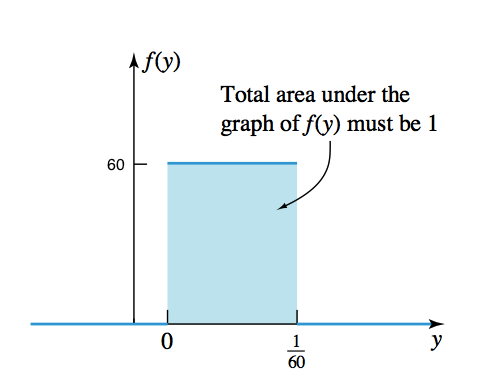
\includegraphics{../../fig/delaypict.png}
\end{frame}

\begin{frame}
\frametitle{Your turn: calculate the following probabilities.}
\begin{align*}
f(y) = \begin{cases}
60 & 0 \le y \le \frac{1}{60} \\
0 & \text{otherwise}
\end{cases}
\end{align*}

\begin{enumerate}[1. ]
\item $P(Y \le \frac{1}{100}$)
\item $P(Y > \frac{1}{70})$
\item $P(|Y| < \frac{1}{120}$)
\item $P(\left |Y - \frac{1}{200} \right | > \frac{1}{110}$)
\item $P(Y = \frac{1}{80}$)
\end{enumerate}
\end{frame}






\begin{frame}<handout:\answers>
\frametitle{Answers: calculate the following probabilities} \small
\begin{enumerate}[1. ]
\item 
\begin{align*}
\uncover<2->{ P(Y \le \frac{1}{100})} &\uncover<2->{  = P(-\infty < Y \le \frac{1}{100})} \\
&\uncover<3->{  = \int_{-\infty}^{1/100} f(y) dy} \\
& \uncover<4->{ = \int_{-\infty}^0 0 dy = \int_{0}^{1/100} 60 dy} \\
& \uncover<5->{ = \frac{60}{100} = \frac{3}{5}}
\end{align*}
\end{enumerate}
\end{frame}




\begin{frame}<handout:\answers>
\begin{enumerate}[1. ]
\setcounter{enumi}{1}
\item 
\begin{align*}
\uncover<2->{ P( Y > \frac{1}{70})} & \uncover<2->{ = P(\frac{1}{70} < Y \le \infty)} \\
&\uncover<3->{ = \int_{1/70}^\infty f(y) dy} \\
&\uncover<4->{ = \int_{1/70}^{1/60} 60 dy + \int_{1/60}^\infty 0 dy} \\
&\uncover<5->{ = 60y \mid_{1/70}^{1/60} + 0} \\
&\uncover<6->{ = 60 \left (\frac{1}{60} - \frac{1}{70} \right )} \\
&\uncover<7->{ = \frac{1}{7} \approx 0.143}
\end{align*}
\end{enumerate}
\end{frame}



\begin{frame}<handout:\answers>
\begin{enumerate}[1. ]
\setcounter{enumi}{2}
\item 
\begin{align*}
\uncover<2->{ P(|Y| < \frac{1}{120})} & \uncover<2->{ = P(-\frac{1}{120} < Y < \frac{1}{120})} \\
&\uncover<3->{ = \int_{-1/120}^{1/120} f(y) dy} \\
& \uncover<4->{ = \int_{-1/120}^0 0 dy + \int_{0}^{1/120} 60 dy} \\
& \uncover<5->{ = 0 + 60y \mid_{0}^{1/120}} \\
& \uncover<6->{ = 60 \left (\frac{1}{120} - 0 \right ) = \frac{1}{2}}
\end{align*}
\end{enumerate}
\end{frame}

\begin{frame}<handout:\answers>
\begin{enumerate}[1. ]
\setcounter{enumi}{3}
\item 
\begin{align*}
\uncover<2->{ P(} &\uncover<2->{  \left |Y - \frac{1}{200} \right | > \frac{1}{110})} \\
&\uncover<3->{ = P(Y - \frac{1}{200} > \frac{1}{110} \text{ or } Y - \frac{1}{200} < -\frac{1}{110})} \\
&\uncover<4->{ = P(Y > \frac{31}{2200} \text{ or } Y < -\frac{9}{2200}) }\\
&\uncover<5->{ = P(Y > \frac{31}{2200}) + P(Y < -\frac{9}{2200})} \\
&\uncover<6->{ = \int_{31/2200}^\infty f(y) dy + \int_{-\infty}^{-9/2200} f(y)dy} \\
&\uncover<7->{ = \int_{31/2200}^{1/60} 60 dy + \int_{1/60}^\infty 0 dy + \int_{-\infty}^{-9/2200} 0 dy} \\
&\uncover<8->{ = 60 |_{31/2200}^{1/60} + 0 + 0} \\
&\uncover<9->{  = 60 \left (\frac{1}{60} - \frac{31}{2200} \right  ) = \frac{17}{6600} \approx 0.00258}
\end{align*}
\end{enumerate}
\end{frame}

\begin{frame}<handout:\answers>

\begin{enumerate}[1. ]
\setcounter{enumi}{4}
\item 

\begin{align*}
\uncover<2->{ P(Y = \frac{1}{80})} &\uncover<2->{ = P(\frac{1}{80} \le Y \le \frac{1}{80})} \\
&\uncover<3->{ = \int_{1/80}^{1/80} f(y) dy = \int_{1/80}^{1/80} 60 dy} \\
&\uncover<4->{ = 60 \mid_{1/80}^{1/80} = 60 \left ( \frac{1}{80} - \frac{1}{80} \right )} \\
&\uncover<5->{  = 0}
\end{align*}

\uncover<6->{ In fact, for any random variable $X$ and any real number $a$:}
\begin{align*}
\uncover<7->{ P(X = a)} &\uncover<8->{ = P(a \le X \le a)} \\
&\uncover<9->{ = \int_a^a f(x) dx} \uncover<10->{  = 0}
\end{align*}
\end{enumerate}
\end{frame}


















\section{Cumulative Distribution Functions}


\begin{frame}
\frametitle{Cumulative distribution functions (cdf)}
\begin{itemize}
\pause \item The {\bf cumulative distribution function} of a random variable $X$ is a function $F$ such that:
\pause \begin{align*}
F(x) &= P(X \le x) = \int_{-\infty}^x f(t) dt\\
 \intertext{\uncover<4->{In other words:}}
\uncover<5->{ \frac{d}{dx}F(x)} &\uncover<5->{= f(x)}
\end{align*}
\uncover<6->{ \item As with discrete random variables, $F$ has the following properties:}
\begin{itemize}
\uncover<7->{ \item $F(x) \ge 0$ for all $x$.}
\uncover<8->{ \item $F$ is monotonically increasing.}
\uncover<9->{ \item $\lim_{x \rt -\infty} F(x)$ = 0}
\uncover<10->{ \item $\lim_{x \rt \infty} F(x)$ = 1}
\end{itemize}
\end{itemize}
\end{frame}

\begin{frame}
\frametitle{Example: calculating the cdf of $Y$} \scriptsize
\begin{itemize}
\pause \item Remember:
\pause \begin{align*}
f_Y(y) = \begin{cases}
60 & \quad 0 < y < 1/60 \\
0 & \quad \text{otherwise}
\end{cases}
\end{align*}
\pause \item For $y \le 0$:
\begin{align*}
\uncover<5->{F(y) } \uncover<5->{=P(Y \le y) =}\uncover<6->{ \int_{-\infty}^y f(t) dt}\uncover<7->{ = \int_{-\infty}^0 0 dt} \uncover<8->{= 0}
\end{align*}
\uncover<9->{\item For $0 < y < 1/60$:}
\begin{align*}
\uncover<10->{F(y)} \uncover<10->{= P(Y \le y)} \uncover<11->{= \int_{-\infty}^y f(t) dt} \uncover<12->{= \int_{-\infty}^0 0 dt + \int_0^y 60 dt} \uncover<13->{= 60y }
\end{align*}
\uncover<14->{\item For $y \ge 1/60$:}
\begin{align*}
\uncover<15->{F(y)} &\uncover<15->{= P(Y \le y)} \uncover<16->{= \int_{-\infty}^y f(t) dt }\\
& \uncover<17->{= \int_{-\infty}^0 0 dt + \int_0^{1/60} 60 dt + \int_{1/60}^{\infty} 0 dt} \uncover<18->{ = 1}
\end{align*}
\end{itemize}
\end{frame}

\begin{frame}
\frametitle{A look at the cdf}
\setkeys{Gin}{width=1\textwidth} 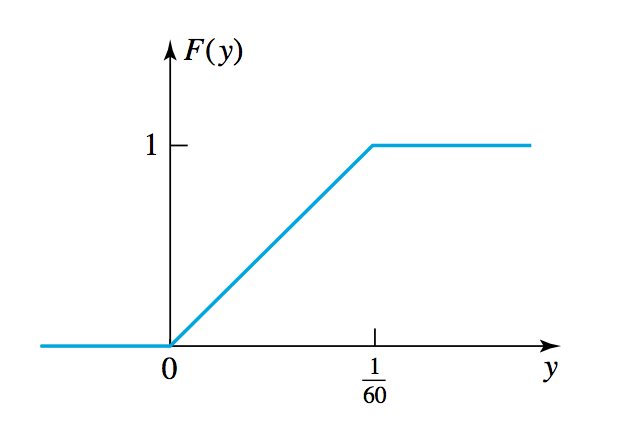
\includegraphics{../../fig/delaycdfpic.png}
\end{frame}

\begin{frame}
\frametitle{Your turn: calculate the following using the cdf}

\begin{align*}
F(y) = \begin{cases}
0 & y \le 0 \\
60y & 0 < y \le \frac{1}{60} \\
1 & y > \frac{1}{60}
\end{cases}
\end{align*}

\begin{enumerate}[1. ]
\item $F({1/70})$
\item $P(Y \le \frac{1}{80})$
\item $P(Y > \frac{1}{150})$
\item $P(\frac{1}{130} \le Y  \le \frac{1}{120})$
\end{enumerate}
\end{frame}






\begin{frame}<handout:\answers>
\frametitle{Answers: calculate the following using the cdf}
\begin{enumerate}[1. ]
\pause \item $F(\frac{1}{70}) = 60 \frac{1}{70} = \frac{6}{7}$
\pause \item $P(Y \le \frac{1}{80}) = F(\frac{1}{80}) = 60 \frac{1}{80} = \frac{3}{4}$
\item \begin{align*}
\uncover<4->{P(Y > \frac{1}{150})} & \uncover<4->{= \int_{1/150}^\infty f(y) dy} \\
& \uncover<5->{= \int_{-\infty}^\infty f(y) dy - \int_{-\infty}^{1/150} f(y)dy} \\
& \uncover<6->{= 1 - F(1/150) = 1 - \frac{60}{150}} \\
& \uncover<7->{= \frac{3}{5}}
\end{align*}
\uncover<8->{In fact, for any random variable $X$, discrete or continuous:}
\begin{align*}
\uncover<9->{P(X \ge x) = 1 - P(X < x)}
\end{align*}
\end{enumerate}
\end{frame}

\begin{frame}
\begin{enumerate}
\setcounter{enumi}{3}
\item 
\begin{align*}
\uncover<2->{P(\frac{1}{130} \le Y  \le \frac{1}{120})} & \uncover<2->{= \int_{1/130}^{1/120} f(y) dy} \\
&\uncover<3->{= \int_{-\infty}^{1/120}f(y) dy - \int_{-\infty}^{1/130}f(y) dy} \\
&\uncover<4->{= F(1/120) - F(1/130)} \\
&\uncover<5->{ = 60 (1/120) - 60(1/130)} \\
& \uncover<6->{= 1/26 \approx 0.0384}
\end{align*}
\end{enumerate}
\end{frame}






\section{A special case: the exponential distribution}

\begin{frame}
\frametitle{The exponential distribution}
\begin{itemize}
\pause \item A random variable $X$ has an Exponential($\alpha$) distribution if:
\pause \begin{align*}
f(x) = \begin{cases}
\frac{1}{\alpha} e^{-x/\alpha} & x > 0 \\
0 & \text{otherwise}
\end{cases}
\end{align*}
\setkeys{Gin}{width=.9\textwidth} \includegraphics<1->{../../fig/expdens.png}
\end{itemize}
\end{frame}

\begin{frame}
\frametitle{Your turn: for $X \sim $ Exp(2), calculate the following}
\begin{align*}
f(x) = \begin{cases}
\frac{1}{2} e^{-x/2} & x > 0 \\
0 & \text{otherwise}
\end{cases}
\end{align*}

\begin{enumerate}[1. ]
\item $P(X  \le 1)$
\item $P(X > 5)$
\item The cdf $F$ of $X$
\end{enumerate}
\end{frame}




\begin{frame}<handout:\answers>
\frametitle{Answers: for $X \sim $ Exp(2), calculate the following}
\begin{enumerate}[1. ]
\item \begin{align*}
\uncover<2->{P(X \le 1)} &\uncover<2->{= \int_{-\infty}^1 f(x) dx} \\
&\uncover<3->{= \int_{-\infty}^0 0 dx +  \int_0^1 \frac{1}{2} e^{-x/2} dx} \\
&\uncover<4->{= 0 + ( -e^{-x/2}\mid_{0}^1} \\
&\uncover<5->{=  -e^{-1/2} - (-  e^{-0/2})} \\
&\uncover<6->{= 1 - e^{-1/2} \approx 0.393}
\end{align*}
\end{enumerate}
\end{frame}

\begin{frame}<handout:\answers>
\begin{enumerate}[1. ]
\setcounter{enumi}{1}
\item \begin{align*}
\uncover<2->{P(X > 5)} & \uncover<2->{= \int_5^\infty f(x) dx} \\
&\uncover<3->{= \int_5 ^\infty \frac{1}{2}e^{-x/2} dx} \\
&\uncover<4->{= -e^{-x/2}|_5^\infty} \\
&\uncover<5->{= -e^{-\infty/2} + e^{-5/2}} \\
&\uncover<6->{= e^{-5/2} \approx 0.082}
\end{align*}
\end{enumerate}
\end{frame}

\begin{frame}<handout:\answers>
\begin{enumerate}[1. ]
\setcounter{enumi}{2}
\item For $x < 0$:
\begin{align*}
\uncover<2->{F(x)} &\uncover<2->{= P(X \le x) = \int_{-\infty}^x f(x) dx)} \\
&\uncover<3->{ = \int_{-\infty}^x 0 dx = 0}
\end{align*}
\uncover<4->{For $x \ge 0$:}
\begin{align*}
\uncover<5->{F(x)} & \uncover<5->{= P(X \le x) = \int_{-\infty}^x f(x)dx} \\
&\uncover<6->{= \int_{-\infty}^0 0 dx + \int_{0}^x \frac{1}{2}e^{-t/2} dt} \\
&\uncover<7->{= -e^{-t/2}\mid_0^x = -e^{-x/2} - (-e^{-0/2})} \\
& \uncover<8->{= 1 - e^{-x/2}}
\end{align*}
\end{enumerate}
\end{frame}

\begin{frame}<handout:\answers>
\begin{align*}
\intertext{Hence:}
\uncover<2->{F(x)} & \uncover<2->{= \begin{cases}
1 - e^{-x/2} & x \ge 0 \\
0 & \text{otherwise}
\end{cases}}
\end{align*}
\uncover<3->{In general, an Exp($\alpha$) random variable has cdf:}
\begin{align*}
\uncover<4->{F(x) = \begin{cases}
1 - e^{-x/\alpha} & x \ge 0 \\
0 & \text{otherwise}
\end{cases}}
\end{align*}
\end{frame}




\begin{frame}
\frametitle{Uses of the Exp($\alpha$) random variable}
\begin{itemize}
\pause \item An Exp($\alpha$) random variable measures the waiting time until a specific event that has an equal chance of happening at any point in time.
\pause \item Examples:
\begin{itemize}
\pause \item Time between your arrival at a bus stop and the moment the bus comes.
\pause \item Time until the next person walks inside the library.
\pause \item Time until the next car accident on a stretch of highway.
\end{itemize}
\end{itemize}
\end{frame}

\end{document}
